%%%%%%%%%%%%  Generated using docx2latex.com  %%%%%%%%%%%%%%

%%%%%%%%%%%%  v2.0.0-beta  %%%%%%%%%%%%%%

\documentclass[12pt]{article}
\usepackage{amsmath}
\usepackage{latexsym}
\usepackage{amsfonts}
\usepackage[normalem]{ulem}
\usepackage{array}
\usepackage{amssymb}
\usepackage{graphicx}
\usepackage[backend=biber,
style=numeric,
sorting=none,
isbn=false,
doi=false,
url=false,
]{biblatex}\addbibresource{bibliography.bib}

\usepackage{subfig}
\usepackage{wrapfig}
\usepackage{wasysym}
\usepackage{enumitem}
\usepackage{adjustbox}
\usepackage{ragged2e}
\usepackage[svgnames,table]{xcolor}
\usepackage{tikz}
\usepackage{longtable}
\usepackage{changepage}
\usepackage{setspace}
\usepackage{hhline}
\usepackage{multicol}
\usepackage{tabto}
\usepackage{float}
\usepackage{multirow}
\usepackage{makecell}
\usepackage{fancyhdr}
\usepackage[toc,page]{appendix}
\usepackage[hidelinks]{hyperref}
\usetikzlibrary{shapes.symbols,shapes.geometric,shadows,arrows.meta}
\tikzset{>={Latex[width=1.5mm,length=2mm]}}
\usepackage{flowchart}\usepackage[paperheight=11.0in,paperwidth=8.5in,left=1.0in,right=1.0in,top=1.0in,bottom=1.0in,headheight=1in]{geometry}
\usepackage[utf8]{inputenc}
\usepackage[T1]{fontenc}
\TabPositions{0.5in,1.0in,1.5in,2.0in,2.5in,3.0in,3.5in,4.0in,4.5in,5.0in,5.5in,6.0in,}

\urlstyle{same}


 %%%%%%%%%%%%  Set Depths for Sections  %%%%%%%%%%%%%%

% 1) Section
% 1.1) SubSection
% 1.1.1) SubSubSection
% 1.1.1.1) Paragraph
% 1.1.1.1.1) Subparagraph


\setcounter{tocdepth}{5}
\setcounter{secnumdepth}{5}


 %%%%%%%%%%%%  Set Depths for Nested Lists created by \begin{enumerate}  %%%%%%%%%%%%%%


\setlistdepth{9}
\renewlist{enumerate}{enumerate}{9}
		\setlist[enumerate,1]{label=\arabic*)}
		\setlist[enumerate,2]{label=\alph*)}
		\setlist[enumerate,3]{label=(\roman*)}
		\setlist[enumerate,4]{label=(\arabic*)}
		\setlist[enumerate,5]{label=(\Alph*)}
		\setlist[enumerate,6]{label=(\Roman*)}
		\setlist[enumerate,7]{label=\arabic*}
		\setlist[enumerate,8]{label=\alph*}
		\setlist[enumerate,9]{label=\roman*}

\renewlist{itemize}{itemize}{9}
		\setlist[itemize]{label=$\cdot$}
		\setlist[itemize,1]{label=\textbullet}
		\setlist[itemize,2]{label=$\circ$}
		\setlist[itemize,3]{label=$\ast$}
		\setlist[itemize,4]{label=$\dagger$}
		\setlist[itemize,5]{label=$\triangleright$}
		\setlist[itemize,6]{label=$\bigstar$}
		\setlist[itemize,7]{label=$\blacklozenge$}
		\setlist[itemize,8]{label=$\prime$}

\setlength{\topsep}{0pt}\setlength{\parindent}{0pt}

 %%%%%%%%%%%%  This sets linespacing (verticle gap between Lines) Default=1 %%%%%%%%%%%%%%


\renewcommand{\arraystretch}{1.3}


%%%%%%%%%%%%%%%%%%%% Document code starts here %%%%%%%%%%%%%%%%%%%%



\begin{document}
\begin{Center}
{\fontsize{16pt}{19.2pt}\selectfont \textbf{H1\_B Visa petition data analysis and approval prediction}\par}
\end{Center}\par

\begin{Center}
Chengnan Xu(cx223), Tian Yu(ty364)
\end{Center}\par


\vspace{\baselineskip}
\begin{FlushLeft}
{\fontsize{14pt}{16.8pt}\selectfont \textbf{1 Problem definition}\par}
\end{FlushLeft}\par

\begin{justify}
In our project, we want to predict the outcome of H1B\_visa applicants based on the dataset. H1\_B visa, non-immigration visa category for international students who want to work in America, is highly desired. It required petition employees at least a bachelor’s degree. As more and more employees go into America, based on Citizenship and Immigration Services(USCIS) grants 85,000 H1\_B visas every year, the visa outcome for the applicants of importance. 
\end{justify}\par

\begin{justify}
The input to our algorithm is based on the dataset features and we will also do some feature engineering such as converted to 0 or 1 for the feature. The output would be the case status whether certified or denied.
\end{justify}\par

{\fontsize{14pt}{16.8pt}\selectfont \textbf{2 About the dataset}\par}\par

\textbf{2.1 Dataset overview}\par

\begin{justify}
Our dataset is from Kaggle listed under the name $``$H-1B Visa Petitions 2011-2016 dataset$"$ . There are 10 features and more than 3 million examples in our dataset. The dataset contains some missing data and the data values are heterogeneous including continuous values, discrete values, nominal data and text. 
\end{justify}\par



%%%%%%%%%%%%%%%%%%%% Figure/Image No: 1 starts here %%%%%%%%%%%%%%%%%%%%

\begin{figure}[H]
	\begin{Center}
		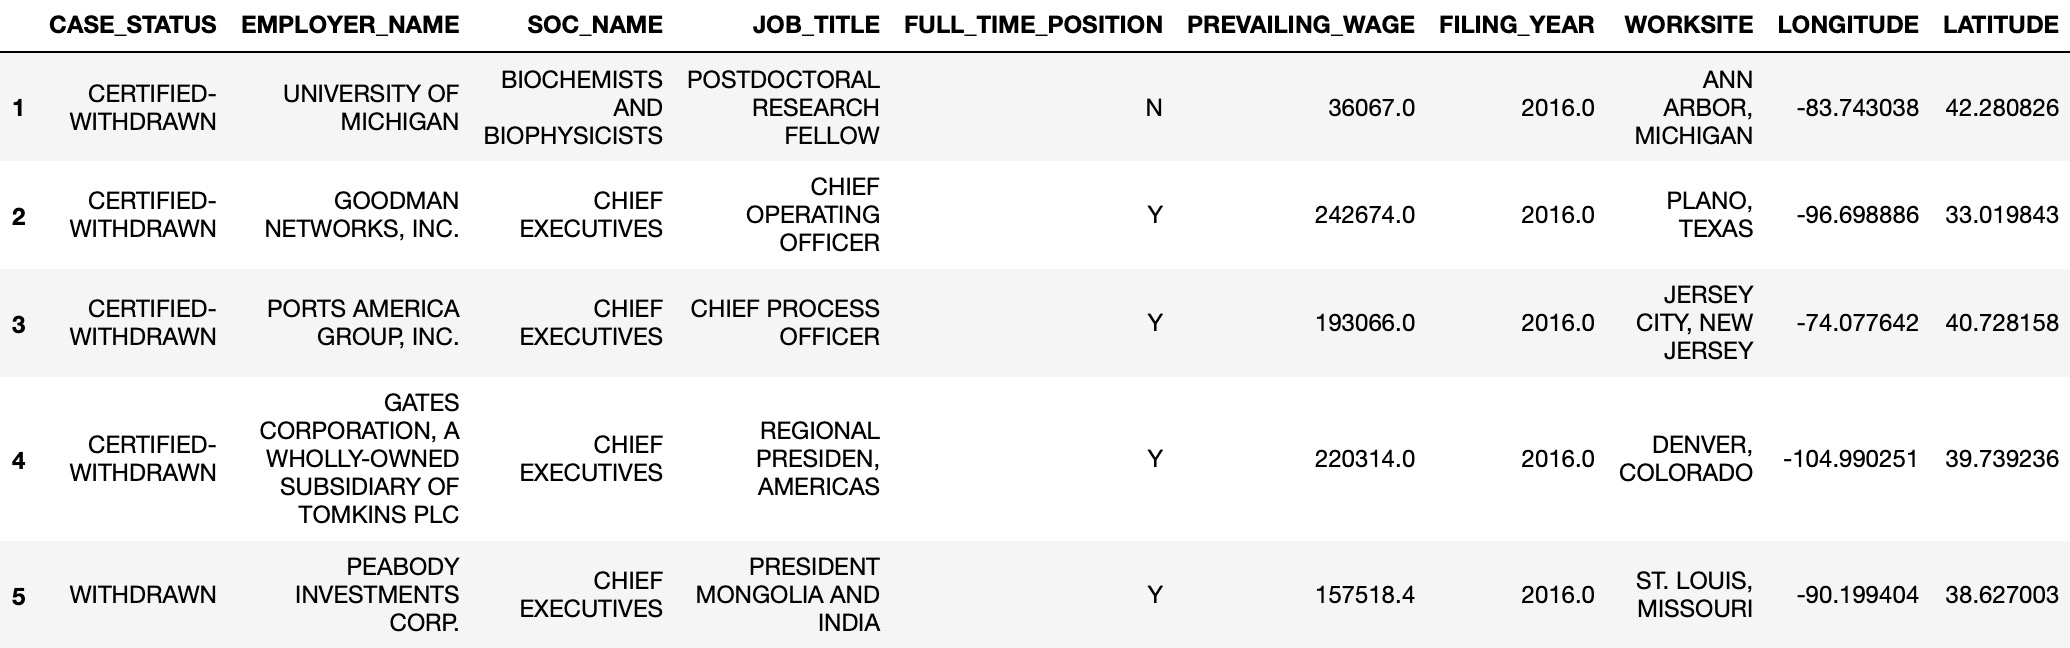
\includegraphics[width=5.16in,height=1.62in]{./media/image1.jpg}
	\end{Center}
\end{figure}


%%%%%%%%%%%%%%%%%%%% Figure/Image No: 1 Ends here %%%%%%%%%%%%%%%%%%%%

\begin{justify}
 
\end{justify}\par

\begin{Center}
{\fontsize{8pt}{9.6pt}\selectfont Fig. 1: First 5 points from the unprocessed dataset\par}
\end{Center}\par


\vspace{\baselineskip}
\begin{justify}
\textbf{2.2 Feature engineering}
\end{justify}\par

\begin{justify}
We\ processed some of the existing features, created new features that we thought could be useful for prediction and discarded some features using the library Pandas. For example, in our training data, some original features like SOC NAME  is not directly related to our CASE\_STATUS, Therefore, we calculated the success rate and total number of applications to create new highly correlated features The detailed explanation is below.
\end{justify}\par

\begin{justify}
CASE\_STATUS: We only maintain ‘CERTIFIED’ and ‘DENIED’ in CASE\_STATUS, with labeled as ‘1’ and ‘0’.
\end{justify}\par

\begin{justify}
FULL\_TIME\_POSITION: For the full time position column, there are two cases, $ \{ $ Y, N$ \} $  for applicants who have full time position or not. We labeled $``$FULL TIME POSITION$"$  = $``$Y$"$  as 1 and $``$FULL TIME POSITION$"$  = $``$N$"$  as 0.
\end{justify}\par

\begin{justify}
EMPLOYER\_ACCEPTANCE:  We created a feature for the ratio of H-1B applicants who were certified per employer. 
\end{justify}\par

\begin{justify}
EMPLOYER\_ACCEPTANCE: Also categorized into six types for ratio of acceptance and converted the data into one-hot-k representation. We created a feature for the success rate per SOC type,converted to one-hot-k representation.
\end{justify}\par

\begin{justify}
JOB\_ACCEPTANCE: We created a feature for the success rate per Job type, converted to one-hot-k representation.
\end{justify}\par

\begin{justify}
WORKSITE:\ For the format of $ \{ $ City, State$ \} $ ,  we only included $"$ State$"$  and converted the data into one-hot-k representation.
\end{justify}\par

\begin{justify}
WAGE\_CATEGRORY: we created a feature for the prevailing wage which is the average wage paid to employees with similar qualifications. Category the average wage into five kinds$ \{ $ very low, low, medium, high, very high$ \} $  and then converted to one-hot-k representation. 
\end{justify}\par

\begin{justify}
FILING\_YEAR:\ \ columns Year the applicants were filed,  we converted data of different year into type int and applied one-hot-k representation.
\end{justify}\par

\begin{justify}
\textbf{2.3 Exploratory data analysis}
\end{justify}\par

\begin{justify}
\tab Our label CASE\_STATUS has seven different categories. To get more information about the CASE\_STATUS, we plot the histogram of case status versus number of petition of the visa petition. 
\end{justify}\par



%%%%%%%%%%%%%%%%%%%% Figure/Image No: 2 starts here %%%%%%%%%%%%%%%%%%%%

\begin{figure}[H]
	\begin{Center}
		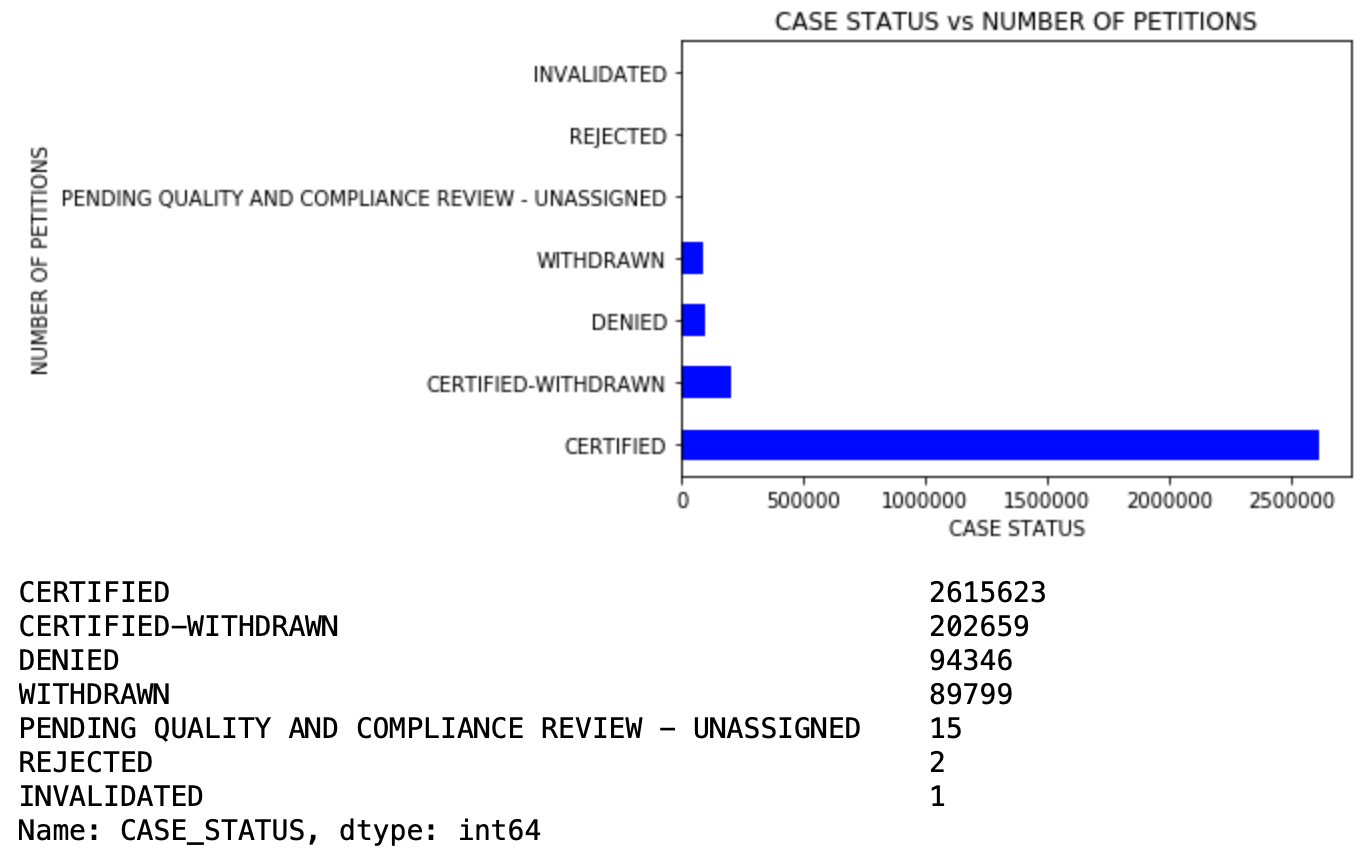
\includegraphics[width=4.89in,height=1.98in]{./media/image5.png}
	\end{Center}
\end{figure}


%%%%%%%%%%%%%%%%%%%% Figure/Image No: 2 Ends here %%%%%%%%%%%%%%%%%%%%

\par

\begin{Center}
{\fontsize{8pt}{9.6pt}\selectfont Fig. 2 the histogram of seven classes in CASE\_STATUS\par}
\end{Center}\par


\vspace{\baselineskip}


%%%%%%%%%%%%%%%%%%%% Figure/Image No: 3 starts here %%%%%%%%%%%%%%%%%%%%


\begin{figure}[H]	\begin{subfigure}		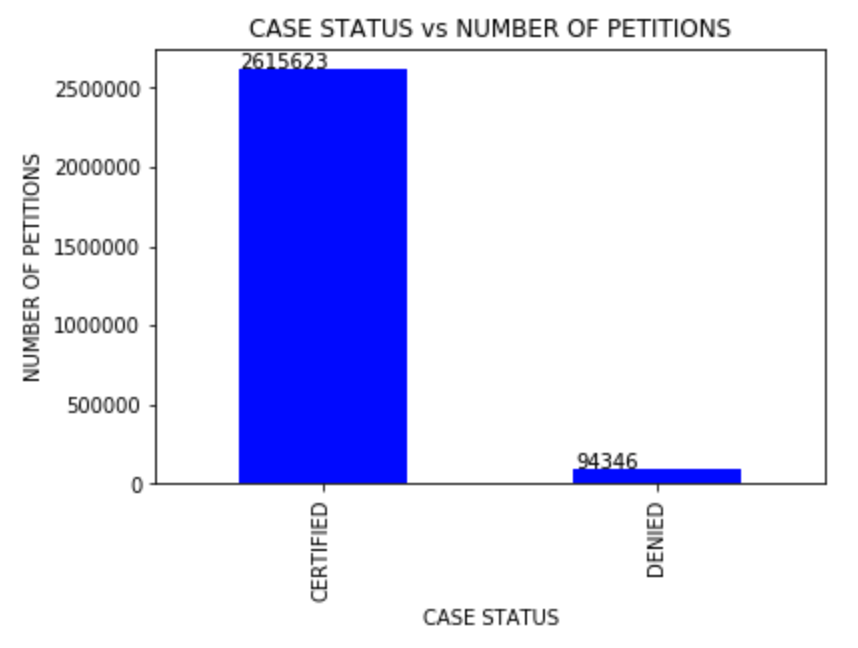
\includegraphics[width=0.45\textwidth]{./media/image3.png}
	\end{subfigure}
~	\begin{subfigure}		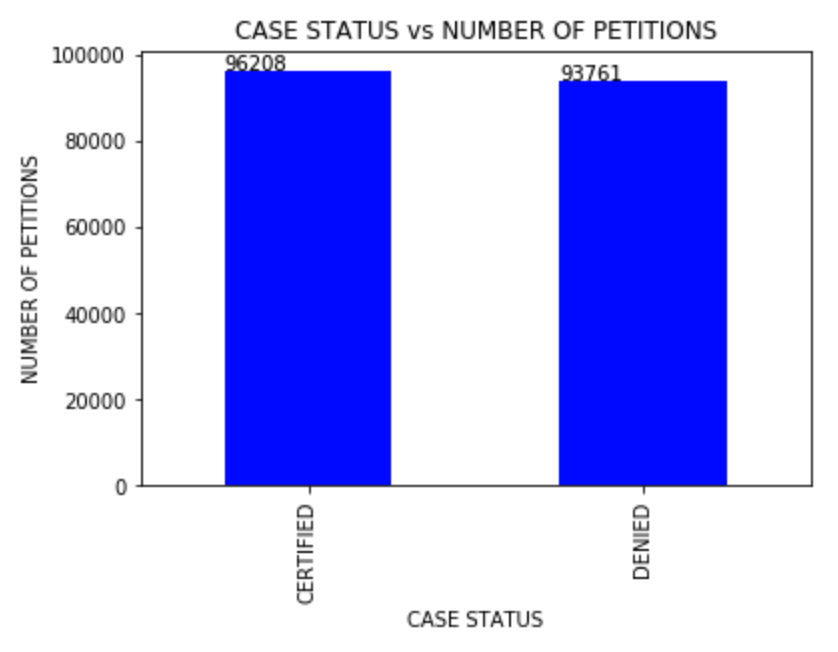
\includegraphics[width=0.45\textwidth]{./media/image2.png}
	\end{subfigure}
~
\end{figure}


%%%%%%%%%%%%%%%%%%%% Figure/Image No: 3 Ends here %%%%%%%%%%%%%%%%%%%%

\par

{\fontsize{8pt}{9.6pt}\selectfont \ \ \ \ \ \ \ \ \ \ \ Fig.3  imbalanced classes in CASE\_STATUS{\fontsize{10pt}{12.0pt}\selectfont \tab \ \ \ \ \ \ \ \ \ \ \ \ \ \ \ \ \ \  {\fontsize{8pt}{9.6pt}\selectfont  Fig.4 equal ratio after undersampling\par}\par}\par}\par


\vspace{\baselineskip}

\vspace{\baselineskip}
\begin{justify}
From\ Fig.1, we observe that the total amount of some CASE\_STATUS outcome classes are relevant quite low. We decided to discard the ‘INVALIDATED,’ ‘REJECTED’, ‘PENDING QUALITY AND COMPLIANCE REVIEW - UNASSIGNED’ class because of the trivial amount.  
\end{justify}\par

\begin{justify}
By applying pandas.dataframe.isnull(), we statistically summarized the missing data in the dataset and we remove rows with null values for $``$EMPLOYER\_NAME$"$ , $``$SOC\_NAME$"$ , $``$JOB\_TITLE$"$ , $``$FULL\_TIME\_POSITION$"$ , $``$PREVAILING\_WAGE$"$  by apply dataframe.dropna
\end{justify}\par

\begin{justify}
We also plot the histogram of CASE\_STATUS vs number of petitions. From Fig.2, we can see the dataset is highly imbalanced, with only 3.5$\%$  of case status being declined. The imbalanced dataset may contribute to model’s overfitting problem, the problem and solution will be elaborated in the preliminary models part.
\end{justify}\par

\tab 
\vspace{\baselineskip}\begin{FlushLeft}
{\fontsize{14pt}{16.8pt}\selectfont \textbf{3 Preliminary Models}\par}
\end{FlushLeft}\par

\begin{FlushLeft}
\textbf{3.1 Overfitting and underfitting}
\end{FlushLeft}\par

\begin{justify}
After the pre-processing steps described above, we split the training and test sets 80:20. Training set had a total of 2.4 million examples. Due to the inherent bias in our dataset towards the $"$ CERTIFIED$"$  label(Fig. 2), the model learning from imbalanced training dataset performed badly in the test datatest. The precision of $``$CERTIFIED$"$  class is up to 95$\%$  while the precision of $``$DENIED$"$  class is lower than 50$\%$  .The model is overfitting.
\end{justify}\par

\begin{justify}
To address imbalanced classes problem, undersampling the majority class is a good choice, especially when we have millions of rows in our project dataset. Undersampling can be defined as removing some observations of the majority class and it can only be applied after splitting test and train set. After resampling, we have an equal ratio of ‘CERTIFIED’ data points to ‘DENIED’ data points(Fig. 3) , but a smaller quantity of data to train machine learning models on.
\end{justify}\par

\textbf{3.2 Decision tree and model effectiveness}\par

\begin{justify}
In order to test our model performance, we calculate the confusion matrix by the help function in the sklearn library. We also used the metric of precision, recall, and f1-score to evaluate the model performance on $``$CERTIFIED$"$  and $``$DENIED$"$  class.
\end{justify}\par



%%%%%%%%%%%%%%%%%%%% Figure/Image No: 4 starts here %%%%%%%%%%%%%%%%%%%%

\begin{figure}[H]
	\begin{Center}
		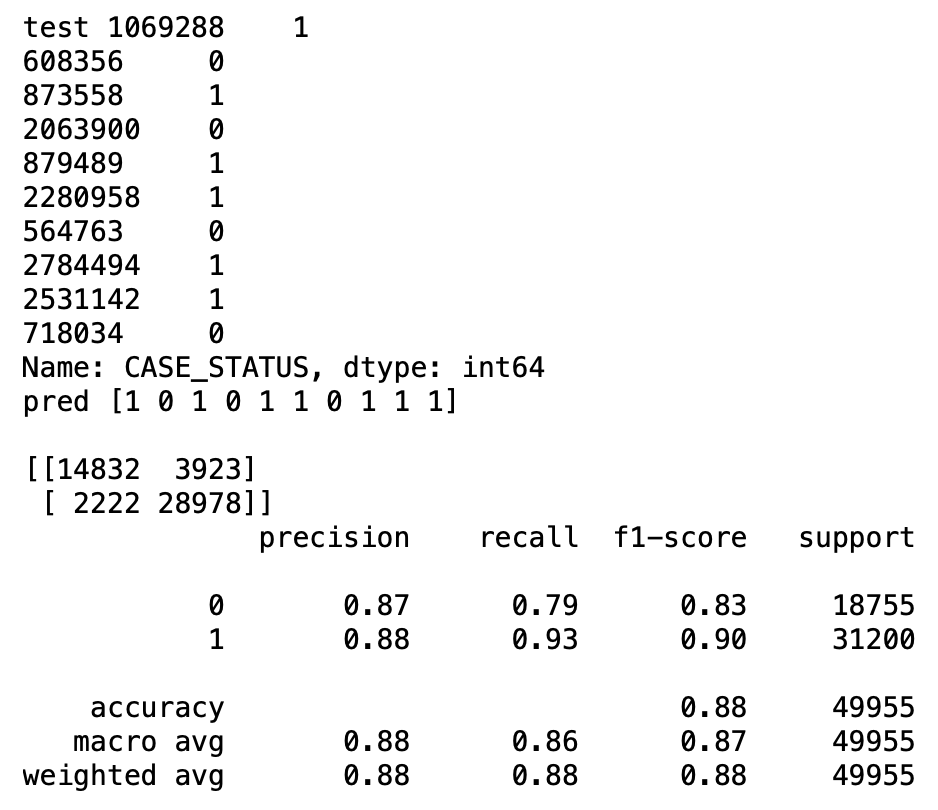
\includegraphics[width=3.69in,height=1.45in]{./media/image4.png}
	\end{Center}
\end{figure}


%%%%%%%%%%%%%%%%%%%% Figure/Image No: 4 Ends here %%%%%%%%%%%%%%%%%%%%

\ \ \ \ \ \ \ \ \ \ \ \ \ \ \ \ \ \ \ \  \par

\begin{Center}
{\fontsize{8pt}{9.6pt}\selectfont Fig.5 the metrics of the decision tree performance\par}
\end{Center}\par

The overall accuracy is about 88 percent.\par


\vspace{\baselineskip}
{\fontsize{14pt}{16.8pt}\selectfont \textbf{4 Next steps}\par}\par

\begin{justify}
Moving forward we will fit alternative models to the dataset such as SVM, random forest, as well as other models. We also want to determine the best prediction model for the data, also apply more techniques we learned in class such as ridge regression or LASSO to help predict better. Besides, we will use like crose validation or included k-fold to help predict well. Comparing with each methods’ performance, we will choose the most optimal one for H1B\_Visa approval prediction for applicants.
\end{justify}\par


\vspace{\baselineskip}

\printbibliography
\end{document}